\subsection{The default definition on the real cohorts}
\label{sec:results-definitions}

Table~\ref{tab:definitions} gives the long-run average PD of S\&P's grades under the four definitions, and Figure~\ref{fig:lra-definitions} shows the same quantities for S\&P and Fitch with the Jeffreys intervals of the pooled counts. The default page and the defaults page agree to within a few percent of each other in every grade, because they count the same distinct defaulted ratings and differ only in the cohort ($\spLraDtwoCcc\%$ and $\spLraDthreeCcc\%$ for CCC to C). The transition page does not agree with them. For CCC to C the long-run average is $\spLraDfourCcc\%$ against $\spLraDtwoCcc\%$, and keeping the withdrawals in the denominator lowers it further to $\spLraKeepCcc\%$. The gap index of Equation~\eqref{eq:gap-index} on the averages is $\spPtRatioCcc$ (the median of its bootstrap distribution is $\spRatioCcc$), with a 95\% bootstrap interval of $\spRatioCccLo$ to $\spRatioCccHi$; the pooled counts say the same thing with sampling error alone, $\spPooledDefDtwoCcc$ defaults over $\spPooledNDtwoCcc$ ratings under the default page ($\spPooledRateDtwoCcc\%$, Jeffreys interval $\spJeffLoDtwoCcc\%$ to $\spJeffHiDtwoCcc\%$) against $\spPooledDefDfourCcc$ over $\spPooledNDfourCcc$ under the transition page ($\spPooledRateDfourCcc\%$, $\spJeffLoDfourCcc\%$ to $\spJeffHiDfourCcc\%$). The two intervals do not overlap. For grade B the index is $\spPtRatioB$ ($\spRatioBLo$ to $\spRatioBHi$): the transition page's average is about half the default page's, but the interval reaches $0.5$ and the claim is not made for that grade. The sign of the gap does not vary: the transition page's rate is below the default page's in $\spYearsBelowCcc$ of $\spYearsCcc$ years for CCC to C and in $\spYearsBelowB$ of $\spYearsB$ for B, as Figure~\ref{fig:yearly-gap} shows year by year. The two series move together: for CCC to C both pages peak in the same year, $\spPeakYearCccDtwo$, at $\spPeakRateCccDtwo\%$ under the default page and $\spPeakRateCccDfour\%$ under the transition page, and the gap persists in the years of low default rates, so it is not the effect of a few recession years.

\begin{table}[htbp]
\centering
\setlength{\tabcolsep}{3.5pt}
\footnotesize
\caption{Long-run average one-year PD (percent) of S\&P's corporate ratings by grade under the four definitions of a default over the 26 annual CEREP cohorts, and the IRB risk weight of the cohort mix; the last column is the ratio of the transition page's average to the default page's with its 95\% bootstrap interval over cohort years (grades with fewer than three nonzero years carry no ratio).}
\label{tab:definitions}
\resizebox{\linewidth}{!}{\begin{tabular}{lrrrrr}
\toprule
Grade & Default page & Defaults page & Transition page & Withdrawals kept & Transition over default page \\
\midrule
\relax AAA & $0.000$ & $0.000$ & $0.000$ & $0.000$ & \relax -- \\
\relax AA & $0.009$ & $0.009$ & $0.005$ & $0.005$ & \relax -- \\
\relax A & $0.035$ & $0.035$ & $0.030$ & $0.029$ & $0.89$ [0.53, 1.08] \\
\relax BBB & $0.113$ & $0.113$ & $0.079$ & $0.075$ & $0.71$ [0.47, 0.96] \\
\relax BB & $0.530$ & $0.541$ & $0.336$ & $0.303$ & $0.63$ [0.47, 0.76] \\
\relax B & $2.957$ & $3.042$ & $1.330$ & $1.163$ & $0.45$ [0.37, 0.53] \\
\relax CCC-C & $26.637$ & $27.577$ & $8.608$ & $5.875$ & $0.32$ [0.26, 0.39] \\
\relax IRB risk weight (\%) & $58.0$ & $58.3$ & $47.5$ & $45.2$ & $10.5$ points \\
\bottomrule
\end{tabular}}
\end{table}


\begin{figure}[htbp]
\centering
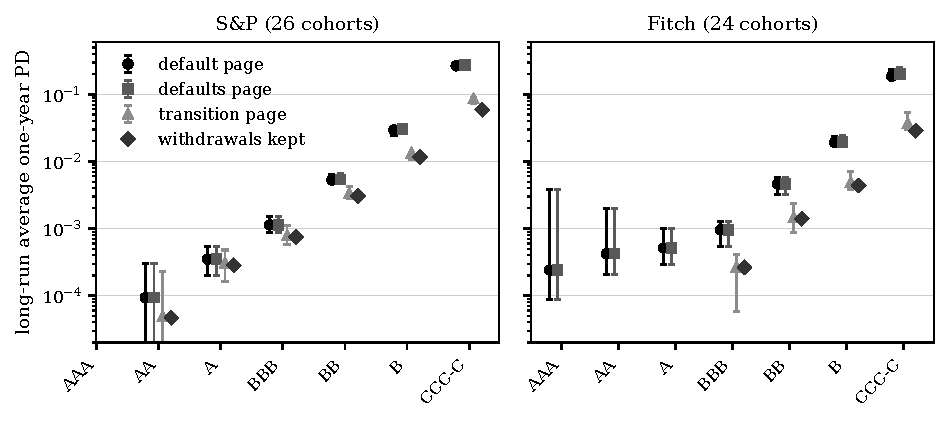
\includegraphics[width=\linewidth]{lra-definitions}
\caption{Long-run average one-year PD by grade of S\&P and Fitch under the default page, the defaults page, the transition page and the transition page with the withdrawals kept, on a logarithmic axis, with the Jeffreys intervals of the pooled counts of the three pages that publish counts; grades with an average of zero are not drawn.}
\label{fig:lra-definitions}
\end{figure}

\begin{figure}[htbp]
\centering
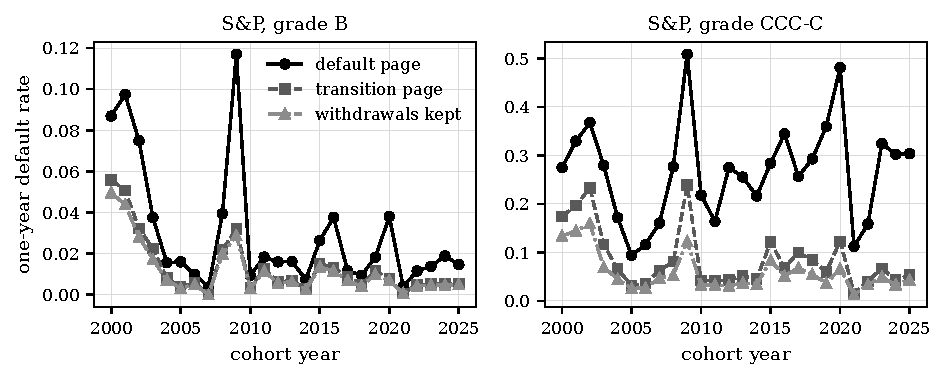
\includegraphics[width=\linewidth]{yearly-gap}
\caption{One-year default rate of S\&P's grades B and CCC to C for each annual cohort from 2000 to 2025 under the default page, the transition page and the transition page with the withdrawals kept, showing that the transition page lies below the default page in every year.}
\label{fig:yearly-gap}
\end{figure}

Figure~\ref{fig:lra-definitions} shows that the gap is largest in the speculative grades, where the withdrawn share and the default rate are both large; in grade A the interval of the gap index of Table~\ref{tab:definitions} includes one, and AA, which has $\spAaNonzeroYears$ year with a nonzero rate, carries no ratio in the table. It does not show why the gap exists. The three explanations that the data cannot separate are the definitions themselves (a rating that defaults and is then withdrawn leaves the transition page's default column), informative withdrawal, and the difference between the cohorts that the pages divide by, which is larger for the default page in $\spGapYears$ of S\&P's years. % voice-ok: withdrawn rating, the domain term of the study

The capital consequence is in Table~\ref{tab:rw} and Figure~\ref{fig:rw-definitions}. The risk weight of S\&P's cohort mix is $\spRwDtwo\%$ with the PDs of the default page and $\spRwDfour\%$ with those of the transition page, a fall of $\spRwGap$ points whose 95\% bootstrap interval is $\spRwGapLo$ to $\spRwGapHi$ and which is positive in $\spRwGapShare\%$ of the $\bootB$ resamples; keeping the withdrawals lowers the weight to $\spRwKeep\%$. For Fitch the weight falls from $\fiRwDtwo\%$ to $\fiRwDfour\%$ ($\fiRwGapLo$ to $\fiRwGapHi$ points), and the transition page's gap index for CCC to C is $\fiPtRatioCcc$ ($\fiRatioCccLo$ to $\fiRatioCccHi$); but these Fitch values carry the defect of the data that Section~\ref{sec:design-data} names: in the $\fiPopDroppedN$ years from \fiPopDropped{} the transition page's default category is empty in every grade, so its rate is zero in those years whatever happened. On the $\fiPopYears$ years in which the category is populated the weight falls from $\fiPopRwDtwo\%$ to $\fiPopRwDfour\%$, a fall of $\fiPopRwGap$ points ($\fiPopRwGapLo$ to $\fiPopRwGapHi$, the last two rows of Table~\ref{tab:rw}), and the gap index for CCC to C is $\fiPopPtRatioCcc$ ($\fiPopRatioCccLo$ to $\fiPopRatioCccHi$), with averages of $\fiPopLraDtwoCcc\%$ and $\fiPopLraDfourCcc\%$. The excess of Fitch's all-years fall over S\&P's is therefore the effect of the empty years, and on the usable years Fitch's gap is of the order of S\&P's. The intervals of the levels overlap in Figure~\ref{fig:rw-definitions}, because the years that raise the rates under one page raise them under the other; the interval of the difference does not, because the resample is common to the definitions. Moody's default page gives $\moLraDtwoCcc\%$ for CCC to C and a weight of $\moRwDtwo\%$, so the default pages of S\&P and Moody's differ by a factor of $\agencyRatio$ for that grade, a spread of the same order as the factor of $\spRatioCccInverse$ that the definitions of S\&P produce. Prediction H1 holds for CCC to C: the upper end of the interval of the gap index is below $0.5$ and the lower end of the risk-weight difference is above zero and above 5 points.

\begin{table}[htbp]
\centering
\setlength{\tabcolsep}{3.5pt}
\footnotesize
\caption{IRB risk weight of each agency's cohort mix (F-IRB corporate, LGD 45\%, maturity 2.5 years, Basel III function) when the one-year PD of every grade is read under each definition, with the percentile interval of 2{,}000 resamples of the cohort years; Moody's transition page has no default category, and the last two rows restrict Fitch to the years in which its transition page's default column is populated.}
\label{tab:rw}
\begin{tabular}{llrrr}
\toprule
Agency & Definition & Risk weight (\%) & 95\% bootstrap interval & Below default page (points) \\
\midrule
\relax S\&P & \relax default page & $58.0$ & \relax [50.0, 65.4] & \relax -- \\
\relax S\&P & \relax defaults page & $58.3$ & \relax [50.3, 65.6] & \relax -- \\
\relax S\&P & \relax transition page & $47.5$ & \relax [40.0, 54.5] & $10.5$ \\
\relax S\&P & \relax withdrawals kept & $45.2$ & \relax [38.2, 52.1] & $12.7$ \\
\relax Moody's & \relax default page & $61.1$ & \relax [49.9, 71.8] & \relax -- \\
\relax Moody's & \relax defaults page & $61.2$ & \relax [50.0, 71.9] & \relax -- \\
\relax Fitch & \relax default page & $46.9$ & \relax [40.7, 56.1] & \relax -- \\
\relax Fitch & \relax defaults page & $47.0$ & \relax [40.9, 56.2] & \relax -- \\
\relax Fitch & \relax transition page & $31.1$ & \relax [26.2, 35.2] & $15.8$ \\
\relax Fitch & \relax withdrawals kept & $30.3$ & \relax [25.5, 34.3] & $16.6$ \\
\relax Fitch & \relax default page, 15 years & $43.8$ & \relax [39.5, 47.7] & \relax -- \\
\relax Fitch & \relax transition page, 15 years & $35.2$ & \relax [30.3, 39.9] & $8.6$ \\
\bottomrule
\end{tabular}
\end{table}


\begin{figure}[htbp]
\centering
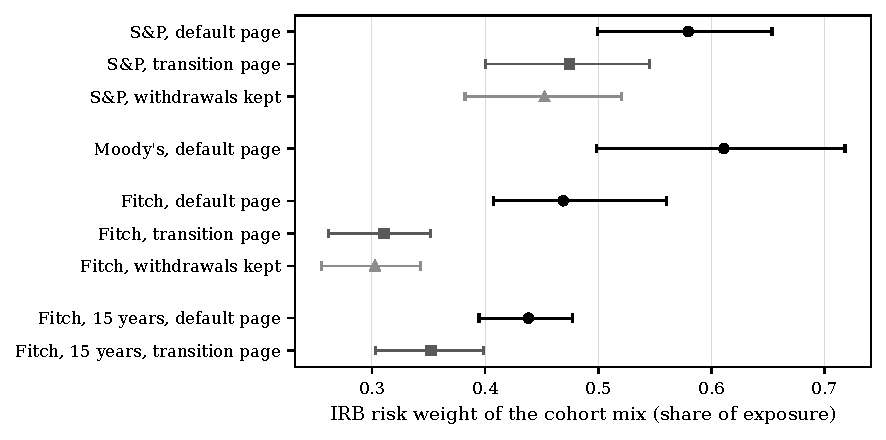
\includegraphics[width=0.92\linewidth]{rw-definitions}
\caption{IRB risk weight of each agency's cohort mix under each definition of the one-year default rate, with the 95\% percentile interval over resamples of the cohort years; Moody's has no transition page default category, so only its default page is shown, and the last two rows restrict Fitch to the years in which its transition page's default category is populated.}
\label{fig:rw-definitions}
\end{figure}

\subsection{Informative withdrawals on paths of known truth}
\label{sec:results-withdrawals}

The committed computation of the case is reproduced to within $\reproMax$ at its four levels of $k$, so the extension rests on the same generator and seeds. Table~\ref{tab:main-results} gives the extension, and Figure~\ref{fig:bias-ladder} plots the bias of grade B against $k$, pooled over five cohorts and on the first cohort alone. At $k=0$, with withdrawal independent of default, removing the withdrawn ratings overstates the PD of B by $\removedBkZero\pm\removedBkZerose$ percent, keeping them understates it by $\keptBkZero\pm\keptBkZerose$ percent, and following them is unbiased ($\followedBkZero\pm\followedBkZerose$), as the first-order formulas predict ($\foRemkZero\%$, $\foKeptkZero\%$ and zero). At $k=1$ the bias of removal has changed sign, $\removedBkOne\pm\removedBkOnese$ percent; at $k=9$, the case the committed computation reports, removal understates the PD by $\removedBkNine\pm\removedBkNinese$ percent, keeping by $\keptBkNine\pm\keptBkNinese$ percent and following by $\followedBkNine\pm\followedBkNinese$ percent (the committed $\repsCommitted$ repetitions gave $\committedremovedkNine\%$, $\committedkeptkNine\%$ and $\committedfollowedkNine\%$). At $k=19$ the removal treatment loses $\removedBkNineteen\pm\removedBkNineteense$ percent of the PD. Grade CCC to C behaves alike: $\removedCcckNine\pm\removedCcckNinese$ percent for removal and $\followedCcckNine\pm\followedCcckNinese$ percent for following at $k=9$. For the lowest grades the estimate is exactly zero in most repetitions (in $\zeroAaaRemoved\%$ of them for AAA with removal at $k=9$), a consequence of the thin cohorts that Section~\ref{sec:results-thin} measures. % voice-ok: withdrawn rating, the domain term of the study

\begin{table}[htbp]
\centering
\setlength{\tabcolsep}{3.5pt}
\footnotesize
\caption{Relative bias (percent of the true one-year PD, mean $\pm$ Monte Carlo standard error over 1{,}000 repetitions) of the pooled cohort estimator with withdrawals removed, kept in the denominator and followed, for grades B and CCC to C, and the error of the IRB risk weight of S\&P's cohort mix (percentage points), against the informativeness $k$ of withdrawal in the year before default.}
\label{tab:main-results}
\resizebox{\linewidth}{!}{\begin{tabular}{rrrrrrrr}
\toprule
$k$ & B removed & B kept & B followed & CCC-C removed & CCC-C followed & Risk weight, removed & Risk weight, followed \\
\midrule
\relax 0 & $2.6\pm0.4$ & $-3.4\pm0.4$ & $-0.2\pm0.4$ & $2.6\pm0.3$ & $-0.3\pm0.3$ & $0.38\pm0.06$ & $-0.09\pm0.06$ \\
\relax 1 & $-2.7\pm0.4$ & $-8.5\pm0.4$ & $-2.3\pm0.4$ & $-1.7\pm0.3$ & $-2.1\pm0.3$ & $-0.42\pm0.06$ & $-0.37\pm0.06$ \\
\relax 2 & $-7.9\pm0.4$ & $-13.4\pm0.3$ & $-4.5\pm0.4$ & $-6.4\pm0.3$ & $-4.5\pm0.3$ & $-1.32\pm0.06$ & $-0.83\pm0.06$ \\
\relax 3 & $-12.0\pm0.4$ & $-17.3\pm0.3$ & $-6.1\pm0.4$ & $-11.2\pm0.3$ & $-7.0\pm0.3$ & $-2.12\pm0.06$ & $-1.15\pm0.06$ \\
\relax 5 & $-20.4\pm0.4$ & $-25.2\pm0.3$ & $-9.2\pm0.4$ & $-19.3\pm0.3$ & $-10.9\pm0.3$ & $-3.55\pm0.06$ & $-1.64\pm0.06$ \\
\relax 9 & $-35.1\pm0.3$ & $-39.2\pm0.3$ & $-15.6\pm0.3$ & $-34.3\pm0.3$ & $-19.0\pm0.3$ & $-6.54\pm0.06$ & $-2.94\pm0.06$ \\
\relax 19 & $-60.3\pm0.3$ & $-62.9\pm0.2$ & $-28.6\pm0.3$ & $-58.9\pm0.2$ & $-33.0\pm0.3$ & $-12.24\pm0.06$ & $-5.35\pm0.06$ \\
\bottomrule
\end{tabular}}
\end{table}


\begin{figure}[htbp]
\centering
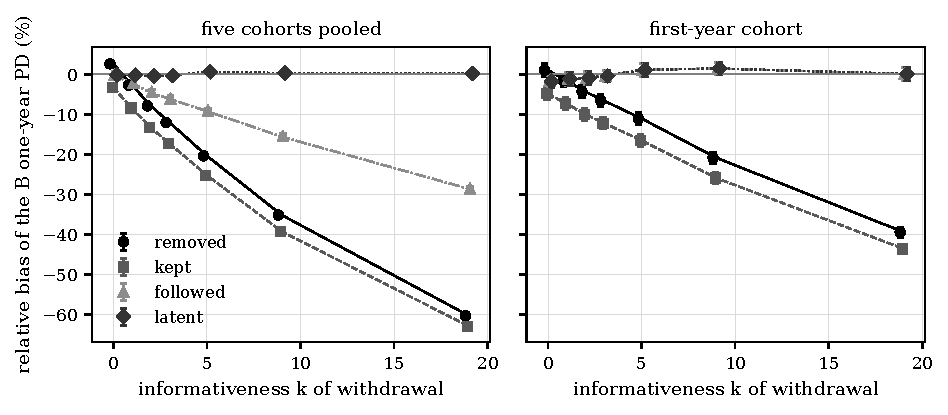
\includegraphics[width=\linewidth]{bias-ladder}
\caption{Relative bias of the one-year PD of grade B against the informativeness of withdrawal for the removal, keeping and following treatments and the no-withdrawal reference, pooled over five annual cohorts (left) and on the first cohort (right), with 95\% intervals from the Monte Carlo standard error of $\repsNew$ repetitions.}
\label{fig:bias-ladder}
\end{figure}

The right panel of Figure~\ref{fig:bias-ladder} is the finding of Proposition~\ref{prop:first-year}. On the first cohort the followed treatment is unbiased at every $k$ (at $k=9$, $\followedYoneBkNine\pm\followedYoneBkNinese$ percent, the sampling noise of the reference), while removal reaches $\removedYoneBkNine\pm\removedYoneBkNinese$ percent and keeping $\keptYoneBkNine\pm\keptYoneBkNinese$ percent. The left panel is the finding of Proposition~\ref{prop:later}: pooling five cohorts adds a bias to the followed treatment that the first cohort did not have. The figure does not show the behaviour of a validator who does not know $k$; the three curves are what each treatment would give at each value of the unknown $k$.

The first-cohort measurements also decide the conjecture of Section~\ref{sec:theory-conjecture}, and they refute it. Table~\ref{tab:conjecture} gives, for the four lowest-rated grades and both treatments, the standardised difference between the measured first-cohort bias and the first-order formula of Equation~\eqref{eq:first-order}. For grade CCC to C the removal treatment differs from the formula by $z=\zCccRemkTwo$, $\zCccRemkFive$ and $\zCccRemkNineteen$ standard errors at $k=2$, $5$ and $19$ (at $k=19$, $\removedYoneCcckNineteen\pm\removedYoneCcckNineteense$ percent against $\foRemkNineteen$ percent); at $k=9$ it is at $z=\zCccRemkNine$, below the criterion of three. For grade B the keeping treatment at $k=19$ differs by $z=\zBKeptkNineteen$ ($\keptYoneBkNineteen\pm\keptYoneBkNineteense$ percent against $\foKeptkNineteen$ percent). Over the grades BBB, BB and B and the levels of $k$ up to nine, the largest difference is $\conjMaxZRestricted$ standard errors over $\conjNRestricted$ comparisons, so that the formula is a usable summary for those grades and levels and not for CCC to C, whose hazard is $\lambdaCcc$ against $\lambdaB$ for B.

\begin{table}[htbp]
\centering
\setlength{\tabcolsep}{3.5pt}
\footnotesize
\caption{Standardised difference $z$ between the measured first-cohort relative bias and the first-order formula of Equation~\eqref{eq:first-order} (measured minus formula, over the Monte Carlo standard error of 1{,}000 repetitions) for the four lowest-rated grades, removal and keeping, at each $k$; a value above three in absolute value, in bold, refutes the conjecture for that case.}
\label{tab:conjecture}
\begin{tabular}{llrrrrrrr}
\toprule
Grade & Treatment & $k=0$ & $k=1$ & $k=2$ & $k=3$ & $k=5$ & $k=9$ & $k=19$ \\
\midrule
\relax BBB & \relax removal & $-0.4$ & $0.1$ & $-0.9$ & $-0.4$ & $-1.2$ & $0.5$ & $-0.0$ \\
\relax BBB & \relax keeping & $-0.4$ & $0.2$ & $-0.9$ & $-0.4$ & $-1.2$ & $0.5$ & $-0.0$ \\
\relax BB & \relax removal & $-0.2$ & $0.0$ & $-0.9$ & $-1.4$ & $-0.7$ & $-1.2$ & $-0.0$ \\
\relax BB & \relax keeping & $-0.2$ & $0.1$ & $-1.0$ & $-1.5$ & $-0.8$ & $-1.3$ & $-0.2$ \\
\relax B & \relax removal & $-2.5$ & $-2.0$ & $-2.0$ & $-1.4$ & $-0.3$ & $-1.0$ & $-1.9$ \\
\relax B & \relax keeping & $-2.5$ & $-2.1$ & $-2.1$ & $-1.6$ & $-0.7$ & $-1.6$ & $\mathbf{-3.1}$ \\
\relax CCC-C & \relax removal & $-1.9$ & $0.1$ & $\mathbf{3.0}$ & $1.2$ & $\mathbf{3.3}$ & $2.8$ & $\mathbf{6.3}$ \\
\relax CCC-C & \relax keeping & $-1.7$ & $-0.1$ & $2.2$ & $0.0$ & $1.2$ & $-0.5$ & $1.0$ \\
\bottomrule
\end{tabular}
\end{table}


The consequence for capital is in the last two columns of Table~\ref{tab:main-results} and in Figure~\ref{fig:rw-error-ladder}. With the true risk weight of the cohort mix at $\rwTruth\%$, the removal treatment lowers it by $\rwAbsremovedkNine$ points at $k=9$ (standard error $\rwremovedkNinese$) and the followed treatment by $\rwAbsfollowedkNine$ points; at $k=19$ the removal error is $\rwremovedkNineteen$ points. The no-withdrawal reference is within $\latentRwMaxZ$ standard errors of zero at every $k$. Prediction H2 holds: at $k=9$ the upper ends of the 95\% intervals of the bias are $\removedBkNine+1.96\times\removedBkNinese$ and $\followedBkNine+1.96\times\followedBkNinese$ percent, both below $-10\%$.

The published estimator that treats a withdrawal as a censoring, the duration estimator, does not escape the bias, as Table~\ref{tab:duration} shows on the same draws. Where withdrawal is independent of default ($k=0$) it is unbiased ($\durBkZero\pm\durBkZerose$ percent for B and $\durCcckZero\pm\durCcckZerose$ for CCC to C, against $\removedBkZero\pm\removedBkZerose$ percent for B with removal), and it estimates a positive PD for AAA ($\zeroAaaDuration\%$ of zero estimates at $k=9$, as at every other level of $k$), where removal returns zero in $\zeroAaaRemoved\%$ of the repetitions at $k=9$. These are the properties for which it is designed. As withdrawal becomes informative it falls below the removal and following treatments, though not below keeping: at $k=9$ it understates the PD of B by $\durBkNine\pm\durBkNinese$ percent and that of CCC to C by $\durCcckNine\pm\durCcckNinese$ percent, against $\removedBkNine\pm\removedBkNinese$ and $\followedBkNine\pm\followedBkNinese$ percent for B under removal and following, and at $k=19$ by $\durBkNineteen\pm\durBkNineteense$ percent; keeping, which divides by the whole cohort, is lower still ($\keptBkNine\pm\keptBkNinese$ percent for B and $\keptCcckNine\pm\keptCcckNinese$ for CCC to C at $k=9$, the kept columns of Table~\ref{tab:duration}). Its bias is thus larger than that of removal and following and smaller than that of keeping. This is the direction expected when withdrawal is more likely before default, a dependence that, as Tsiatis shows, the observed data cannot reveal: the censored paths carry no information on the defaults that the withdrawn ratings would have had, and an estimator that takes the censoring as independent of default cannot recover them. The duration estimator therefore does not repair the bias that the cohort treatments show; the Aalen-Johansen estimator, which makes the same assumption, is not run. % voice-ok: withdrawn rating, the domain term of the study

\begin{table}[htbp]
\centering
\setlength{\tabcolsep}{3.5pt}
\footnotesize
\caption{The duration estimator, which treats a withdrawal as a censoring of the continuous-time path, against the pooled cohort treatments on the same 1{,}000 paired draws: relative bias (percent, mean $\pm$ Monte Carlo standard error) for grades B and CCC to C, and the share of repetitions in which the estimated PD of AAA is exactly zero.}
\label{tab:duration}
\resizebox{\linewidth}{!}{\begin{tabular}{rrrrrrrr}
\toprule
$k$ & B removed & B followed & B duration & CCC-C removed & CCC-C duration & AAA zero, removed (\%) & AAA zero, duration (\%) \\
\midrule
\relax 0 & $2.6\pm0.4$ & $-0.2\pm0.4$ & $-0.4\pm0.3$ & $2.6\pm0.3$ & $-0.3\pm0.3$ & $98.0$ & $0.0$ \\
\relax 1 & $-2.7\pm0.4$ & $-2.3\pm0.4$ & $-5.0\pm0.3$ & $-1.7\pm0.3$ & $-4.9\pm0.3$ & $99.1$ & $0.0$ \\
\relax 2 & $-7.9\pm0.4$ & $-4.5\pm0.4$ & $-10.3\pm0.3$ & $-6.4\pm0.3$ & $-9.6\pm0.3$ & $98.4$ & $0.0$ \\
\relax 3 & $-12.0\pm0.4$ & $-6.1\pm0.4$ & $-14.8\pm0.3$ & $-11.2\pm0.3$ & $-14.0\pm0.3$ & $98.7$ & $0.0$ \\
\relax 5 & $-20.4\pm0.4$ & $-9.2\pm0.4$ & $-22.7\pm0.3$ & $-19.3\pm0.3$ & $-22.1\pm0.3$ & $99.3$ & $0.0$ \\
\relax 9 & $-35.1\pm0.3$ & $-15.6\pm0.3$ & $-37.2\pm0.3$ & $-34.3\pm0.3$ & $-36.8\pm0.2$ & $98.8$ & $0.0$ \\
\relax 19 & $-60.3\pm0.3$ & $-28.6\pm0.3$ & $-61.5\pm0.2$ & $-58.9\pm0.2$ & $-60.8\pm0.2$ & $99.3$ & $0.0$ \\
\bottomrule
\end{tabular}}
\end{table}


\begin{figure}[htbp]
\centering
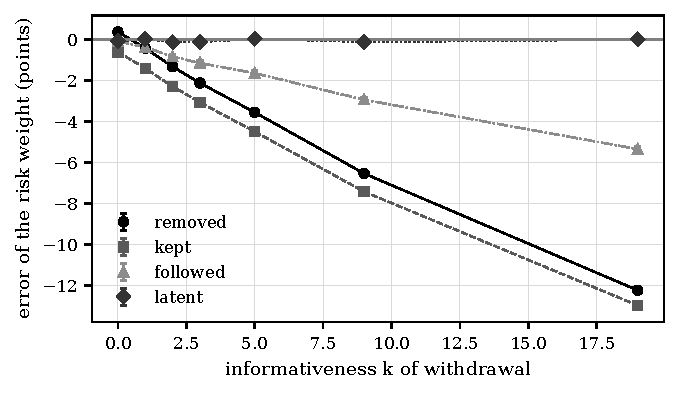
\includegraphics[width=0.72\linewidth]{rw-error-ladder}
\caption{Error, in points, of the IRB risk weight of S\&P's cohort mix computed from the PDs of each treatment of the withdrawn ratings against the informativeness of withdrawal, with 95\% intervals from the Monte Carlo standard error of $\repsNew$ repetitions.} % voice-ok: withdrawn rating, the domain term of the study
\label{fig:rw-error-ladder}
\end{figure}

\subsection{What the transition tests see}
\label{sec:results-tests}

Table~\ref{tab:tests} gives the rejection rates of five transition tests at three levels of $k$ over $\repsTests$ repetitions on the same draws, and Figure~\ref{fig:tests-rejection} plots the first two. At $k=0$ the test of time homogeneity rejects $\testthkZerofive\%$ of the repetitions at the 5\% level (Wilson interval $\testthkZerofivelo$ to $\testthkZerofivehi$) and the test of the last matrix against the true one $\testmrkZerofive\%$ ($\testmrkZerofivelo$ to $\testmrkZerofivehi$), below its level. At $k=9$, where the treatments are $\removedBkNine\%$ and $\followedBkNine\%$ off the truth, the rates are $\testthkNinefive\%$ ($\testthkNinefivelo$ to $\testthkNinefivehi$) and $\testmrkNinefive\%$ ($\testmrkNinefivelo$ to $\testmrkNinefivehi$): the first is within the size of the test plus a fraction, and the second, which compares one year with the truth, is conservative, although its interval at $k=9$ does not overlap its interval at $k=0$, so that it registers a change that it does not turn into a rejection. Neither interval reaches 10\%, so prediction H3 holds as it was stated for these two tests. The three further tests give the following rates at $k=0$, $9$ and $19$: the test of the Markov order $\testordkZerofive\%$, $\testordkNinefive\%$ and $\testordkNineteenfive\%$ (at $k=9$ the Wilson interval is $\testordkNinefivelo$ to $\testordkNinefivehi$, whose upper end is above 10\%), the momentum test $\testmomkZerofive\%$, $\testmomkNinefive\%$ and $\testmomkNineteenfive\%$, and the monotonicity z-tests $\testztkZerofive\%$, $\testztkNinefive\%$ and $\testztkNineteenfive\%$; the Wilson intervals of each of the three overlap across the three levels of $k$. At $k=19$, where removal loses $\removedBkNineteen\%$ of the PD, the time-homogeneity test rejects $\testthkNineteenfive\%$ and the test of the last matrix $\testmrkNineteenfive\%$ ($\testmrkNineteenfivelo$ to $\testmrkNineteenfivehi$), and only then does a test see something. The statement that the prediction rests on, that no matrix test sees the withdrawals, is therefore not held: the test of the last matrix sees them at $k=19$, at a rate whose interval lies well above 10\%. The tests see the withdrawals late, when the bias is already above half the PD, and then at a low rate.

\begin{table}[htbp]
\centering
\setlength{\tabcolsep}{3.5pt}
\footnotesize
\caption{Rejection rates, in percent, of five transition tests of the engine on five annual matrices of the withdrawal generator, over 1{,}000 repetitions per $k$ with Wilson intervals, the same draws for every test at a given $k$; the first two tests are the case's, the other three were run after them, once their results were known. At the level of the test a rate near 5 or 1 means the test does not see the withdrawals; the matrix weighted bandwidth, a descriptive metric with no rejection rule, is not run.}
\label{tab:tests}
\begin{tabular}{lrrr}
\toprule
Transition test & $k$ & Rejections at 5\% (Wilson 95\%) & Rejections at 1\% (Wilson 95\%) \\
\midrule
\relax time homogeneity & \relax 0 & $2.8$ [1.9, 4.0] & $0.4$ [0.2, 1.0] \\
\relax time homogeneity & \relax 9 & $5.8$ [4.5, 7.4] & $1.0$ [0.5, 1.8] \\
\relax time homogeneity & \relax 19 & $8.8$ [7.2, 10.7] & $2.1$ [1.4, 3.2] \\
\relax last year against $\exp(Q)$ & \relax 0 & $0.2$ [0.1, 0.7] & $0.0$ [0.0, 0.4] \\
\relax last year against $\exp(Q)$ & \relax 9 & $1.4$ [0.8, 2.3] & $0.0$ [0.0, 0.4] \\
\relax last year against $\exp(Q)$ & \relax 19 & $16.3$ [14.1, 18.7] & $4.3$ [3.2, 5.7] \\
\relax Markov order & \relax 0 & $6.0$ [4.7, 7.6] & $2.2$ [1.5, 3.3] \\
\relax Markov order & \relax 9 & $8.3$ [6.7, 10.2] & $2.5$ [1.7, 3.7] \\
\relax Markov order & \relax 19 & $6.6$ [5.2, 8.3] & $3.2$ [2.3, 4.5] \\
\relax rating momentum & \relax 0 & $4.2$ [3.1, 5.6] & $0.7$ [0.3, 1.4] \\
\relax rating momentum & \relax 9 & $4.2$ [3.1, 5.6] & $0.8$ [0.4, 1.6] \\
\relax rating momentum & \relax 19 & $4.1$ [3.0, 5.5] & $0.5$ [0.2, 1.2] \\
\relax monotonicity z-tests & \relax 0 & $0.0$ [0.0, 0.4] & $0.0$ [0.0, 0.4] \\
\relax monotonicity z-tests & \relax 9 & $0.0$ [0.0, 0.4] & $0.0$ [0.0, 0.4] \\
\relax monotonicity z-tests & \relax 19 & $0.1$ [0.0, 0.6] & $0.0$ [0.0, 0.4] \\
\bottomrule
\end{tabular}
\end{table}


\begin{figure}[htbp]
\centering
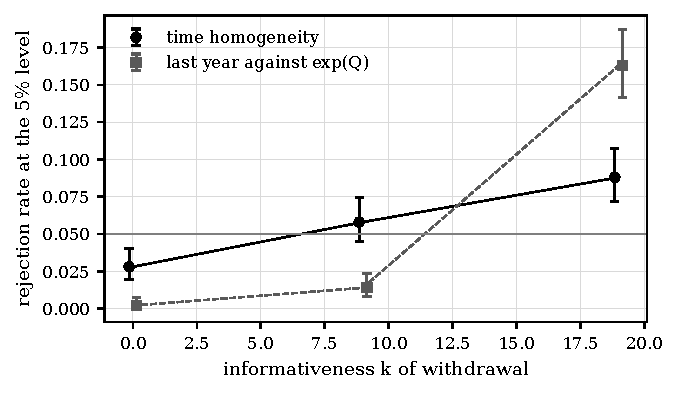
\includegraphics[width=0.72\linewidth]{tests-rejection}
\caption{Rejection rate at the 5\% level of the test of time homogeneity across five annual matrices and of the test of the last matrix against the true one-year matrix, against the informativeness of withdrawal, with Wilson intervals over $\repsTests$ repetitions; the horizontal line is the level of the test.}
\label{fig:tests-rejection}
\end{figure}

\subsection{Thin grades by exact enumeration}
\label{sec:results-thin}

Table~\ref{tab:thin} and Figure~\ref{fig:thin-coverage} give the exact coverage. With 50 obligors per grade the Wald interval contains the PD of AAA in $\waldAaaFifty\%$ of the samples ($\waldAaaFiftyFour\%$ to four digits), of AA in $\waldAaFifty\%$, and in $\waldBbbFifty\%$ of BBB, $\waldBFifty\%$ of B and $\waldCccFifty\%$ of CCC to C. The Agresti-Coull and Jeffreys intervals cover at least $\acMinFifty\%$ and $\jeffMinFifty\%$ in every grade at that size, so the statement of H4 is reproduced in both clauses (the case's committed enumeration is the source of these values, and nothing in this paper's own computation could have refuted them). The price is the width: at the PD of AAA the expected lengths at 50 obligors are $\lenWaldAaaFifty$ basis points for the Wald interval, $\lenJeffAaaFifty$ for the Jeffreys interval and $\lenAcAaaFifty$ for the Agresti-Coull interval, against a PD of $\pAaaBp$ basis points. At 1,000 obligors the Wald interval covers the PD of AAA in $\waldAaaThou\%$ of the samples, and the Jeffreys interval covers $\jeffThouAaa\%$ for AAA, $\jeffThouBb\%$ for BB, $\jeffThouB\%$ for B and $\jeffThouCcc\%$ for CCC to C, below the nominal level, and $\jeffThouAa\%$, $\jeffThouA\%$ and $\jeffThouBbb\%$ for AA, A and BBB, at or above it, as Table~\ref{tab:thin} shows. The shortfall therefore does not follow the thinness of the grade: it falls on AAA and on three of the thicker grades and spares AA, the grade with the lowest PD, because the coverage of the Jeffreys interval oscillates with the number of obligors, the behaviour that Brown, Cai and DasGupta describe for the interval \citep{Brown_2001}. At the cohort sizes of the generator the Wald coverage is $\waldAaaGen\%$ for AAA, $\waldAaGen\%$ for AA and $\waldAGen\%$ for A. The grid of Figure~\ref{fig:thin-coverage} locates the size at which the Wald interval reaches 90\%: $\waldFirstBb$ obligors for BB, $\waldFirstCcc$ for CCC to C, and for AAA no size of the grid up to $\gridMax$ obligors (at $\gridMax$ the coverage is $\waldAaaFiftyK\%$). The grades cannot be told apart in the investment range: at 1,000 obligors the Jeffreys intervals of AAA and AA overlap with probability $\overlapAaaAaThou$, while B and CCC to C separate from 200 obligors (overlap $\overlapBCccTwo$).

\begin{table}[htbp]
\centering
\setlength{\tabcolsep}{3.5pt}
\footnotesize
\caption{Exact coverage (percent, nominal 95) of the Wald, Agresti-Coull and Jeffreys intervals at the true one-year PD of each grade, by enumeration of the binomial count, with 50 and 1{,}000 obligors per grade and at the cohort sizes of the S\&P-like generator; the PDs are those of the C04 generator.}
\label{tab:thin}
\resizebox{\linewidth}{!}{\begin{tabular}{lrrrrrrrrrr}
\toprule
Grade & $p$ (\%) & Wald, 50 & A-C, 50 & Jeffreys, 50 & Wald, 1000 & A-C, 1000 & Jeffreys, 1000 & Cohort size & Wald, size & Jeffreys, size \\
\midrule
\relax AAA & $0.007$ & $0.3$ & $100.0$ & $99.7$ & $6.4$ & $100.0$ & $93.6$ & \relax 75 & $0.5$ & $99.5$ \\
\relax AA & $0.005$ & $0.2$ & $100.0$ & $99.8$ & $4.8$ & $100.0$ & $95.2$ & \relax 822 & $4.0$ & $96.0$ \\
\relax A & $0.029$ & $1.4$ & $100.0$ & $98.6$ & $25.1$ & $99.7$ & $96.6$ & \relax 1814 & $40.7$ & $98.4$ \\
\relax BBB & $0.082$ & $4.0$ & $99.9$ & $96.0$ & $55.8$ & $99.0$ & $95.0$ & \relax 1756 & $76.1$ & $98.4$ \\
\relax BB & $0.346$ & $15.9$ & $99.9$ & $98.7$ & $85.7$ & $97.5$ & $94.4$ & \relax 1054 & $87.5$ & $94.1$ \\
\relax B & $1.173$ & $44.5$ & $97.9$ & $97.9$ & $93.9$ & $96.1$ & $94.6$ & \relax 1391 & $92.5$ & $95.6$ \\
\relax CCC-C & $8.062$ & $91.4$ & $95.5$ & $96.8$ & $94.7$ & $95.2$ & $94.5$ & \relax 201 & $92.6$ & $94.6$ \\
\bottomrule
\end{tabular}}
\end{table}


\begin{figure}[htbp]
\centering
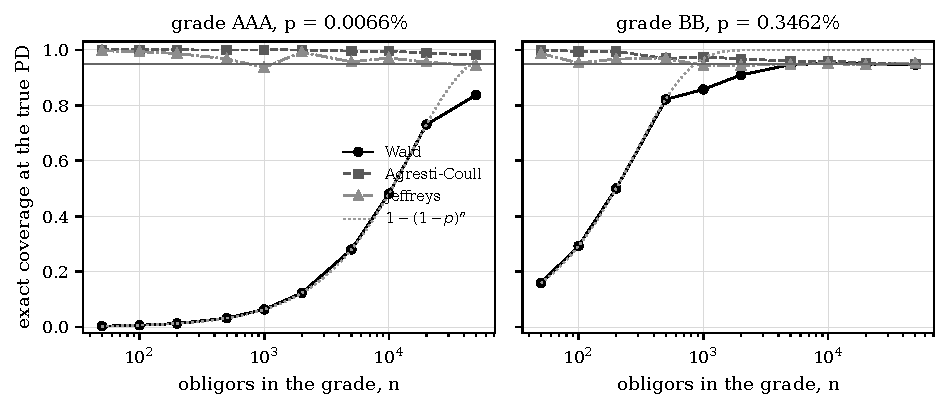
\includegraphics[width=\linewidth]{thin-coverage}
\caption{Exact coverage at the true PD of the Wald, Agresti-Coull and Jeffreys intervals against the number of obligors in the grade, for AAA (left) and BB (right), with the closed form $1-(1-p)^n$ of the Wald coverage as a dotted line and the nominal 95\% as a horizontal line.}
\label{fig:thin-coverage}
\end{figure}

\subsection{The closed forms and the numerical evaluations against the simulation}
\label{sec:results-theory}

Table~\ref{tab:theory} and Figure~\ref{fig:theory-vs-simulation} compare the closed forms of Section~\ref{sec:theory} with the engine's simulation on the two-state chain with the PD of grade B. The largest standardised difference is $\thMaxZFirst$ over the $\thNcmpFirst$ distinct first-cohort comparisons, which test the closed forms of Proposition~\ref{prop:first-year} (H5a), and $\thMaxZPooled$ over the $\thNcmpPooled$ pooled comparisons, which test the numerical evaluation of the model's masses and not a closed form (H5b); the two chains, five levels of $k$, four estimators including the reference and two scopes make $\thNcmp$ entries, of which $\thNcmpDistinct$ are distinct because the first-cohort followed estimator and the reference read the same draws and have the same value. Predictions H5a and H5b hold. The two-state chain does not carry over to the multi-state grades in one direction, and the direction differs between grades. For grade B, the two-state numerical evaluation for the removal treatment pooled over five cohorts at $k=9$ is $\thBremovedPoolkNine\%$, against $\removedBkNine\pm\removedBkNinese\%$ on the multi-state generator of S\&P-like cohorts ($\zTwoStateremovedB$ standard errors apart), whereas for following it gives $\thBfollowedPoolkNine\%$ against $\followedBkNine\pm\followedBkNinese\%$ ($\zTwoStatefollowedB$ standard errors), so that the two-state evaluation overstates the selection bias of the followed treatment. For grade CCC to C it goes the other way for both treatments: removal $\thCccremovedPoolkNine\%$ against $\removedCcckNine\pm\removedCcckNinese\%$ ($\zTwoStateremovedCcc$ standard errors) and following $\thCccfollowedPoolkNine\%$ against $\followedCcckNine\pm\followedCcckNinese\%$ ($\zTwoStatefollowedCcc$ standard errors), that is, the two-state evaluation understates the bias. The sign of the two-state error therefore differs between grade B and grade CCC to C, and the two-state model is a guide to the mechanism and not a substitute for the measurement on the grade at hand. The figure shows the agreement between the closed forms and the two-state simulation for the three treatments in both scopes.

\begin{table}[htbp]
\centering
\setlength{\tabcolsep}{3.5pt}
\footnotesize
\caption{The closed forms of the Theory section (first cohort) and the numerical evaluation of the model's masses (pooled over five cohorts) against the engine's simulation on a two-state chain with the PD of grade B (relative bias of the one-year PD in percent; the simulated value is the mean $\pm$ Monte Carlo standard error of 40 paired draws of 100{,}000 obligors, $z$ the standardised difference).}
\label{tab:theory}
\resizebox{\linewidth}{!}{\begin{tabular}{rlrrrrrr}
\toprule
$k$ & Estimator & Pooled: numerical evaluation & Pooled: simulated & $z$ & First year: closed form & First year: simulated & $z$ \\
\midrule
\relax 0 & \relax removed & $3.0$ & $3.0\pm0.2$ & $0.02$ & $3.0$ & $2.9\pm0.5$ & $-0.28$ \\
\relax 0 & \relax kept & $-2.9$ & $-2.9\pm0.2$ & $0.04$ & $-2.9$ & $-3.1\pm0.4$ & $-0.26$ \\
\relax 0 & \relax followed & $0.0$ & $0.0\pm0.2$ & $0.08$ & $0.0$ & $-0.2\pm0.5$ & $-0.35$ \\
\relax 1 & \relax removed & $-2.2$ & $-2.0\pm0.2$ & $1.06$ & $0.1$ & $-0.2\pm0.4$ & $-0.72$ \\
\relax 1 & \relax kept & $-7.9$ & $-7.7\pm0.2$ & $1.13$ & $-5.8$ & $-6.0\pm0.4$ & $-0.64$ \\
\relax 1 & \relax followed & $-2.2$ & $-2.1\pm0.2$ & $0.83$ & $0.0$ & $-0.3\pm0.4$ & $-0.87$ \\
\relax 3 & \relax removed & $-11.8$ & $-11.7\pm0.2$ & $0.46$ & $-5.4$ & $-5.3\pm0.5$ & $0.16$ \\
\relax 3 & \relax kept & $-17.1$ & $-17.0\pm0.2$ & $0.43$ & $-11.1$ & $-11.0\pm0.5$ & $0.13$ \\
\relax 3 & \relax followed & $-6.5$ & $-6.5\pm0.1$ & $0.05$ & $0.0$ & $0.1\pm0.5$ & $0.18$ \\
\relax 9 & \relax removed & $-35.0$ & $-35.2\pm0.2$ & $-1.18$ & $-19.7$ & $-19.7\pm0.4$ & $0.05$ \\
\relax 9 & \relax kept & $-39.0$ & $-39.2\pm0.2$ & $-1.16$ & $-24.8$ & $-24.7\pm0.4$ & $0.06$ \\
\relax 9 & \relax followed & $-17.4$ & $-17.7\pm0.2$ & $-1.59$ & $0.0$ & $-0.1\pm0.5$ & $-0.18$ \\
\relax 19 & \relax removed & $-60.0$ & $-59.9\pm0.1$ & $0.39$ & $-37.5$ & $-37.4\pm0.4$ & $0.28$ \\
\relax 19 & \relax kept & $-62.6$ & $-62.5\pm0.1$ & $0.39$ & $-41.7$ & $-41.6\pm0.4$ & $0.25$ \\
\relax 19 & \relax followed & $-30.9$ & $-30.8\pm0.2$ & $0.15$ & $0.0$ & $0.8\pm0.5$ & $1.69$ \\
\bottomrule
\end{tabular}}
\end{table}


\begin{figure}[htbp]
\centering
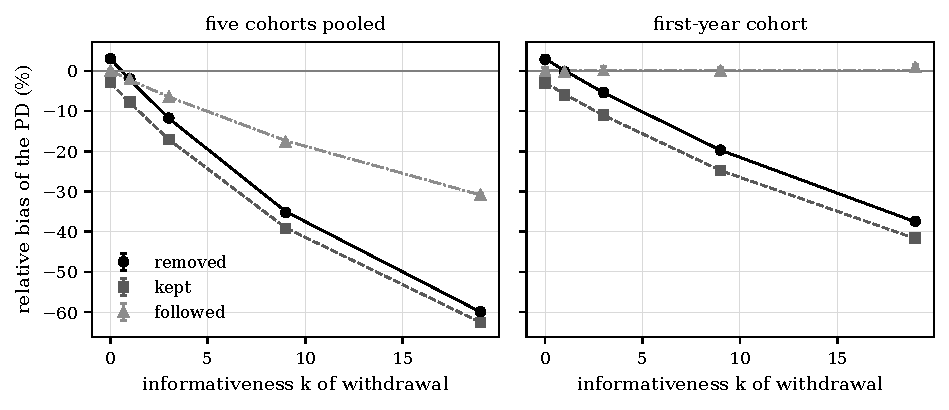
\includegraphics[width=\linewidth]{theory-vs-simulation}
\caption{Relative bias of the one-year PD of a two-state chain with the PD of grade B against the informativeness of withdrawal: the numerical evaluations (pooled, left) and the closed forms (first cohort, right) of the Theory section as lines and the means of the engine's simulation as points with 95\% intervals, pooled over five cohorts (left) and on the first cohort (right).}
\label{fig:theory-vs-simulation}
\end{figure}

\subsection{Outcome of the predictions}
\label{sec:results-outcomes}

Table~\ref{tab:outcomes} lists the predictions and the conjecture with their deciding quantity and their outcome. H1, H2 and the two parts of H5 hold; H4 is reproduced and could not have failed; H3 holds for the two tests at $k=9$ for which it was stated, but the statement behind it does not, because the test of the last matrix rejects in $\testmrkNineteenfive\%$ of the repetitions at $k=19$; and the conjecture is refuted for CCC to C and, at $k=19$, for keeping in grade B. Four details temper the reading. The gap index of grade B at S\&P is not below one half with confidence, so the claim of H1 is made for CCC to C only. The first-order formula of Equation~\eqref{eq:first-order} is refuted for grade CCC to C at three of the seven levels of $k$ (and at $k=9$ it is just under the criterion), and the exact closed form is needed there. The two-state numerical evaluation misses the multi-state followed treatment in both grades, in opposite directions. And the Jeffreys interval, which satisfies the statement of H4 at 50 obligors, is below its nominal coverage at 1,000 obligors in the grades AAA, BB, B and CCC to C, and above it in AA, A and BBB. The outcomes therefore support the statement that the three conventions move the PD, but they support the sharper claims only within the conditions listed: a speculative grade for the gap, a level of informativeness at or above one for the sign of the bias, a PD of about $1.2\%$ or less and a level of informativeness up to nine for the first-order formula, and a cohort whose expected default count is below one for the shortfall of the Wald coverage.

\begin{table}[htbp]
\centering
\setlength{\tabcolsep}{3.5pt}
\footnotesize
\caption{The predictions of the experimental design and the outcome of each: the four statements of the measurements on the default definition, informative withdrawals and thin grades, the closed forms of the Theory section, and the conjecture of that section, with the quantity that decides each.}
\label{tab:outcomes}
\begin{tabular}{lp{5.2cm}p{4.2cm}p{2.6cm}}
\toprule
Id & Prediction & Result & Outcome \\
\midrule
\relax H1 & \relax On S\&P's CEREP cohorts the transition page's long-run PD of CCC to C is below one half of the default page's (95\% interval of the ratio below 0.5), and the risk weight of the cohort mix falls by more than 5 points & $0.323$ [0.259, 0.391]; $10.5$ points [8.3, 13.1] & \relax held (the point values reproduce the committed ones; the bootstrap interval is new) \\
\relax H2 & \relax With $k=9$ the pooled B PD with withdrawals removed and with withdrawals followed are each at least 10\% below the truth (95\% interval of the relative bias below $-10$\%) & \relax removed $-35.1\pm0.3$, followed $-15.6\pm0.3$ & \relax held \\
\relax H3 & \relax At $k=9$ neither the test of time homogeneity nor the test of the last matrix rejects more than 10\% of the repetitions at the 5\% level (upper Wilson bound below 10\%). The statement behind it, that no transition test of the engine sees the withdrawals, is refuted by a rate whose lower bound is above 10\% at any $k$ or any test & $k=9$: $5.8$ [4.5, 7.4] and $1.4$ [0.8, 2.3]; last matrix at $k=19$: $16.3$ [14.1, 18.7]; Markov order at $k=9$: $8.3$ [6.7, 10.2] & \relax held for the two tests at $k=9$; the statement is not held, the last-matrix test sees the withdrawals at $k=19$ \\
\relax H4 & \relax With 50 obligors the Wald interval covers the PD of AAA in $0.33\%$ of the samples (to two digits) and the Jeffreys and Agresti-Coull intervals cover at least 95\% in every grade & \relax Wald $0.33$\%; minimum $96.0$\% (Jeffreys), $95.5$\% (A-C) & \relax reproduced (an exact enumeration of values already committed; it could not fail) \\
\relax H5a & \relax The closed forms of Proposition~\ref{prop:first-year} agree with the simulated means of the first cohort within three Monte Carlo standard errors & \relax largest $|z|=1.69$ over 30 distinct comparisons & \relax held \\
\relax H5b & \relax The numerical evaluation of the model's masses over five cohorts, with the horizon truncation, agrees with the pooled simulated means within three Monte Carlo standard errors & \relax largest $|z|=1.59$ over 40 distinct comparisons & \relax held \\
\relax Conj. & \relax The first-order formula of Equation~\eqref{eq:first-order} describes the first-cohort bias of a grade with a small PD to within three standard errors & \relax CCC to C, removal: $z=3.02$, $3.31$, $6.32$ at $k=2,5,19$; B, keeping, $k=19$: $z=-3.07$ & \relax refuted for CCC to C and, at $k=19$, for keeping in B \\
\bottomrule
\end{tabular}
\end{table}

